\documentclass[
	msc,
	english
%% Para dissertações de mestrado, OU
%	mscproposta, %% Para propostas de dissertação de mestrado, OU
%	phd, %% Para teses de doutorado, OU
%	phdproposta, %% Para propostas de tese de doutorado
%	portugues %% Para documentos em português, OU
%	english %% Para documentos em inglês
]{ppgccufmg}

%\usepackage[brazil]{babel} %% se o documento for em português, OU
\usepackage[english]{babel} %% se o documento for em inglês
%\usepackage[latin1]{inputenc}
\usepackage{natbib}
\usepackage{xcolor}
\usepackage{lipsum}
\usepackage[
	colorlinks=true,
	linkcolor=blue, %% Cor dos links do sumário
	citecolor=red, %% Cor dos links das citações      
	urlcolor=magenta, %% Cor das urls
]{hyperref}

%% Exemplo de lista customizada ==================
%% Para criar uma lista customizada (como Lista de Algoritmos, Lista de Exemplos) que ficará juntamente com as Lista de Figuras e Lista de Tabelas, execute os 3 comandos abaixo substituindo "algoritmos" pelo tipo de lista que estará criando. Para adicionar a lista ao documento, deverá passar o seguinte parâmetro no comando \ppgccufmg:
%% \ppgccufmg{
%% 		...
%% 		listacustomizada={\listadealgoritmos}
%% }
\newfloat[chapter]{algoritmo}{lol}{Algoritmo}
\newcommand{\listaalgoritmosname}{Lista de Algoritmos} %% Título da lista
\newlistof{listadealgoritmos}{lol}{\listaalgoritmosname} %% O primeiro parâmetro é o nome da lista, e este deverá ser passado no parâmetro listacustomizada={\nomedalista}
\newlistentry{algoritmo}{lol}{0} %% Nome do ambiente de cada algoritmo, e.g., \begin{algoritmo} ... \end{algoritmo}

%% **** Caso não haja nenhuma lista adicional, os comandos acima podem ser apagados. ****
%% ===============================================

\begin{document}
	\ppgccufmg{
		autor={Tomaz Gomes Mascarenhas}, %% Autor(a)
		titulopt={Demonstrando teoremas em Lean por meio da reconstrução de provas em SMT},
		tituloen={Proving Lean theorems via reconstructed SMT proofs}, %% Título em inglês
		cidade={Belo Horizonte},
		ano={2023},
		versaopt={Final},
		versaoen={Final}, %% Palavra que acompanhará 'Version' na folha de rosto em inglẽs
		orientador={Haniel Barbosa}, %% Para masculino
		fichacatalografica={fichacatalografica.pdf},
		folhadeaprovacao={folhadeaprovacao.pdf},
		resumo={resumo.tex}, %% Resumo em português
		palavraschave={Verifica\c{c}\~ao Formal, Lean, SMT},
		abstracten={abstract.tex}, %% Abstract em inglês
		keywords={Formal Verification, Lean, SMT}, %% Palavras-chave do abstract
		dedicatoria={dedicatoria.tex}, %% Arquivo .tex contendo a dedicatória
		agradecimentos={agradecimentos.tex},
		epigrafe={S\'o quem sonha acordado v\^e o sol nascer.},
		epigrafeautor={Unknown},
		listadefiguras={sim}, %% Remova (ou comente) este parâmetro para remover a lista de figuras
		listadetabelas={sim}, %% Remova (ou comente) este parâmetro para remover a lista de tabelas
		listascustomizadas={\listadealgoritmos} %% Lista customizada (e.g., lista de algoritmos). 
	}

	\chapter{Introduction}
	  \section{Context}
	    A mechanized proof is a proof, written in some language recognized by a computer, that had its validity checked by a trusted verifier. One of the main applications of these artifacts are formalizing mathematical theories. Indeed, there are well-known examples of successful formalizations. One of them is the mechanization of the proof of a theorem regarding Perfectoid Spaces\cite{scholze}, done by the fields-medalist mathematician Peter Scholze, together with the community of a system called Lean\cite{lean}. Scholze proved the theorem using pen and paper, but was unsure of the result due to its complexity. Once he translated the theorem and the proof to the language of Lean, the system could point out some mistakes he made, and, after fixing them, he could be sure of the correctness of the proof.

Another application of mechanized proofs is verifying the correctness of mission-critical software. Given a specification of the behavior of some program, the program is said to be correct if it respects the specification for any input it is given. For instance, one could specify that a sorting routine must always produce the sorted permutation of it's input list. In this case, a given sorting routine is said to be correct if it indeed produces the desired permutation, regardless of which list it receives. There are a variety of techniques to obtain correctness evidence for a software. The most common one is the development of tests. Besides being easy to write an efficient set of tests, there are many types of bugs that can be discovered with its execution. In fact, this approach is enough for a large amount of problems that are solved by software engineering. However, tests can’t guarantee that a program doesn’t have flaws, since the number of valid inputs is almost always exceedingly large, or infinite. This kind of guarantee is extremely important for mission-critical software, that is, systems that have critical responsibilities, such as the control of airplanes or medical equipment. In this context, one promising alternative is to use a mechanized proof of the correctness of the software as an evidence for its safety.

The process of generating mechanized proofs can be divided into
two categories: interactive and automatic.

Interactive theorem provers (ITPs) are mainly represented by proof assistants, in which, after defining
a theorem, the user attempts to manually write a proof for it,
relying on the tool to organize the set of hypothesis and
how the goal changed step-wisely through the proof, as well as to ensure the
correctness of each step according to a trusted kernel.
%
In order to keep the kernel simple and small (and, therefore, easy to be trusted), it's implementation usually just straightforwardly checks the logic rules from the logic implemented by the ITP.\ Because of this, each step must be explicitly stated by the user, making the tool costly to be used.
% %
% Each logic step must be explicitly stated by the user, which makes the tool
% costly to be used.

Automatic theorem provers (ATPs), on the other hand,
only require the user to define a conjecture, proceeding automatically to
determine whether there exists a proof for it, or possibly providing a
counter-example if it can find one.
%
Although they are easier to use, ATPs require a large
codebase to implement all the algorithms necessary to execute the search for a proof,
making them more susceptible to errors and harder to be trusted.
One possible way to overcome this trust issue is to produce
a mechanized proof verifying the correctness of the ATP, however,
besides being a very complex task, once the proof is done the
development of the ATP becomes freezed, otherwise it would
have to be verified again.

Another approach to increase the confidence in ATPs is to have them provide a
proof to support their results, so that it can be independently verified whether
it indeed proves the theorem in question. This has the downside of creating a need
for allocating resources to verify the proof of every single theorem that is proved.
On the other hand, as long as the proof format doesn't change, the implementation
of the solver can be modified without requiring a modification in the checkers. Also,
it is important to consider that it is often simpler to verify proofs than to verify
the tool itself.

Another important advantage of the second approach is that it allows the ITPs to leverage the automatic proving performed by the ATPs by using the proofs they produce, since the requirement for accepting a proof, i.e.\ that each step is correct to its internal logic,
can be applied to the ATP proof.
%
By connecting these systems, it would be possible for the user of the ITP to focus on more complex steps of the proof, such as defining an induction hypothesis, while delegating the burden of other long and straightforward steps to the ATP.\ Indeed, this
connection is so important that there are projects like Hammering Towards QED~\cite{hammering}
that outline all the efforts that were already made in order to integrate
interactive and automatic theorem provers. In this paper, the authors describe in detail each component that a system that creates a connection between ATPs and ITPs has to implement, as well as the main issues that they have to solve, based on existing programs that were successful in this task. Besides that, they show their potential through several large benchmarks. 


	  \section{Related Work}
	    \subsection{SMTCoq}
			One notable example of such integrations is SMTCoq~\cite{smtcoq}.
It is a plugin for the proof assistant Coq~\cite{Bertot2004} that
can be used as a tactic to prove theorems via their encoding into
SMT and by lifting proofs produced by the SMT solvers veriT~\cite{Bouton2009}
and CVC4~\cite{Barrett2011}. The tool relies on a preprocessor written in OCaml
to transform proof witnesses coming from different solvers into certificates in
the Coq language. The system has a set of checkers for each theory in SMT, each
one of them consisting of theorems asserting the validity of certain transformations
in the SMT terms. All those checkers are connected by the main checker, that
is essentially a theorem stating that if all the transformations resulted in an
empty clause, then the lifting of the original term is false, for any instantiation
of its free variables. This kind of reasoning is known as proof by computational
reflection~\cite{reflection} which is an instance of Certified Transformations, which will be described
in Section~\ref{sec:certifiedVsCertifying}.

		\subsection{Sledgehammer}
			The ITP Isabelle/HOL~\cite{Nipkow2002} has a similar tool,
namely, Sledgehammer~\cite{sledgehammer}. This system achieves its goal by
invoking several SMT solvers in parallel to prove a given goal and collecting
their output to determine which lemmas must be applied in order to prove the theorem
inside Isabelle. In a way, this approach is very similar to the one we're using in this project, as the proof is produced on
the fly (known as the Certifying approach, which will also be described in Section~\ref{sec:certifiedVsCertifying}) as opposed
to having a single theorem that establishes once and for all
that, if all steps performed by the solver were successful,
then the original goal is valid, as is done by SMTCoq.

	  \section{Contributions}
	    Given this context, we present a set of tools that would be an essential
part of the integration between the ITP Lean 4~\cite{lean} and the SMT solver cvc5~\cite{cvc5}.
%
Specifically, we aim to build a system that takes proofs of the unsatisfiability of
SMT queries produced by cvc5 and reconstructs them in Lean.
%
The main motivation of this project is that despite the fact that Lean is
emerging as a promising programming language and proof assistant and being
widely used by mathematicians in large-scale
formalizations~\cite{mathlib, scholze}, there is currently no way to
interact with SMT solvers from it, even though these systems have been
central in previous developments of proof automation in ITPs, as we will show in Sections~\ref{sec:smtcoq}
and~\ref{sec:sledgehammer}. The contribution of the present work
would enable a faster development of this kind of project using Lean.

We use the cvc5 solver because it already has a module for exporting proofs as
Lean scripts~\cite{Barbosa2022}, using a representation of the SMT terms\footnote{For more details
about the SMT term language, see SMT-LIB~\cite{smtlib}.} as an inductive type in Lean.
However, these proofs are not fully verified by Lean's checker. Instead, a set of
axioms are declared in Lean, representing all the logical rules that cvc5 uses to prove
theorems, and the ITP only checks whether the rules were applied correctly and whether
the end result of applying all the rules in the proof is, indeed, the required one.
Our main contributions are to eliminate the need of increasing the trusted base by introducing
those axioms and to make the proofs operate over native Lean terms, as opposed to terms
of the inductive type that represents SMT terms.

Note that the set of tools we are proposing does not implement the full integration
between Lean and cvc5. For instance, we do not implement a module for translating
Lean goals into an equivalent SMT problem. However, our project is being used
as part of the joint project Lean-SMT\footnote{The code for the project can be found at \url{https://github.com/ufmg-smite/lean-smt}}, that aims to implement a tactic in Lean
that would perform the complete process, that is, starting from a Lean goal, translating it to a SMT query, invoking a solver to try to prove it and lifting the proof produced (in case it is found) to Lean's language, so that it can be used as a proof for the original goal.

	\chapter{Formal Preliminaries}
	  \section{Satisfiability Modulo Theories}
	  \section{Lean's Type Theory}
	  \section{Lean's Framework for Metaprogramming}
	\chapter{Certifying Reconstruction of SMT Proofs in Lean}
	  \section{Certified vs Certifying}
	  \section{Tactics}
	  \section{The Complete Architecture}
	  \section{Skipping the Parser}
	  % maybe think of other optimizations and make a section about this
	\chapter{Evaluation}
	\chapter{Future Work}

	% \chapter{Introdução}
	% 	a introducao vem aqui
	% \chapter{Desenvolvimento}
	% 	\lipsum[1-4]

	% 	\begin{algoritmo}
	% 		\centering
	% 		\framebox[.5\textwidth]{\texttt{Código, Código, Código}}
	% 		\caption{Este é o meu Algoritmo 1.}
	% 		\label{alg:algoritmo1}
	% 	\end{algoritmo}

	% 	\begin{algoritmo}
	% 		\centering
	% 		\framebox[.7\textwidth]{\texttt{Mais Código, Mais Código, Mais Código}}
	% 		\caption{Este é o meu Algoritmo 2.}
	% 		\label{alg:algoritmo2}
	% 	\end{algoritmo}

	% 	\begin{figure}[h]
	% 		\centering
	% 		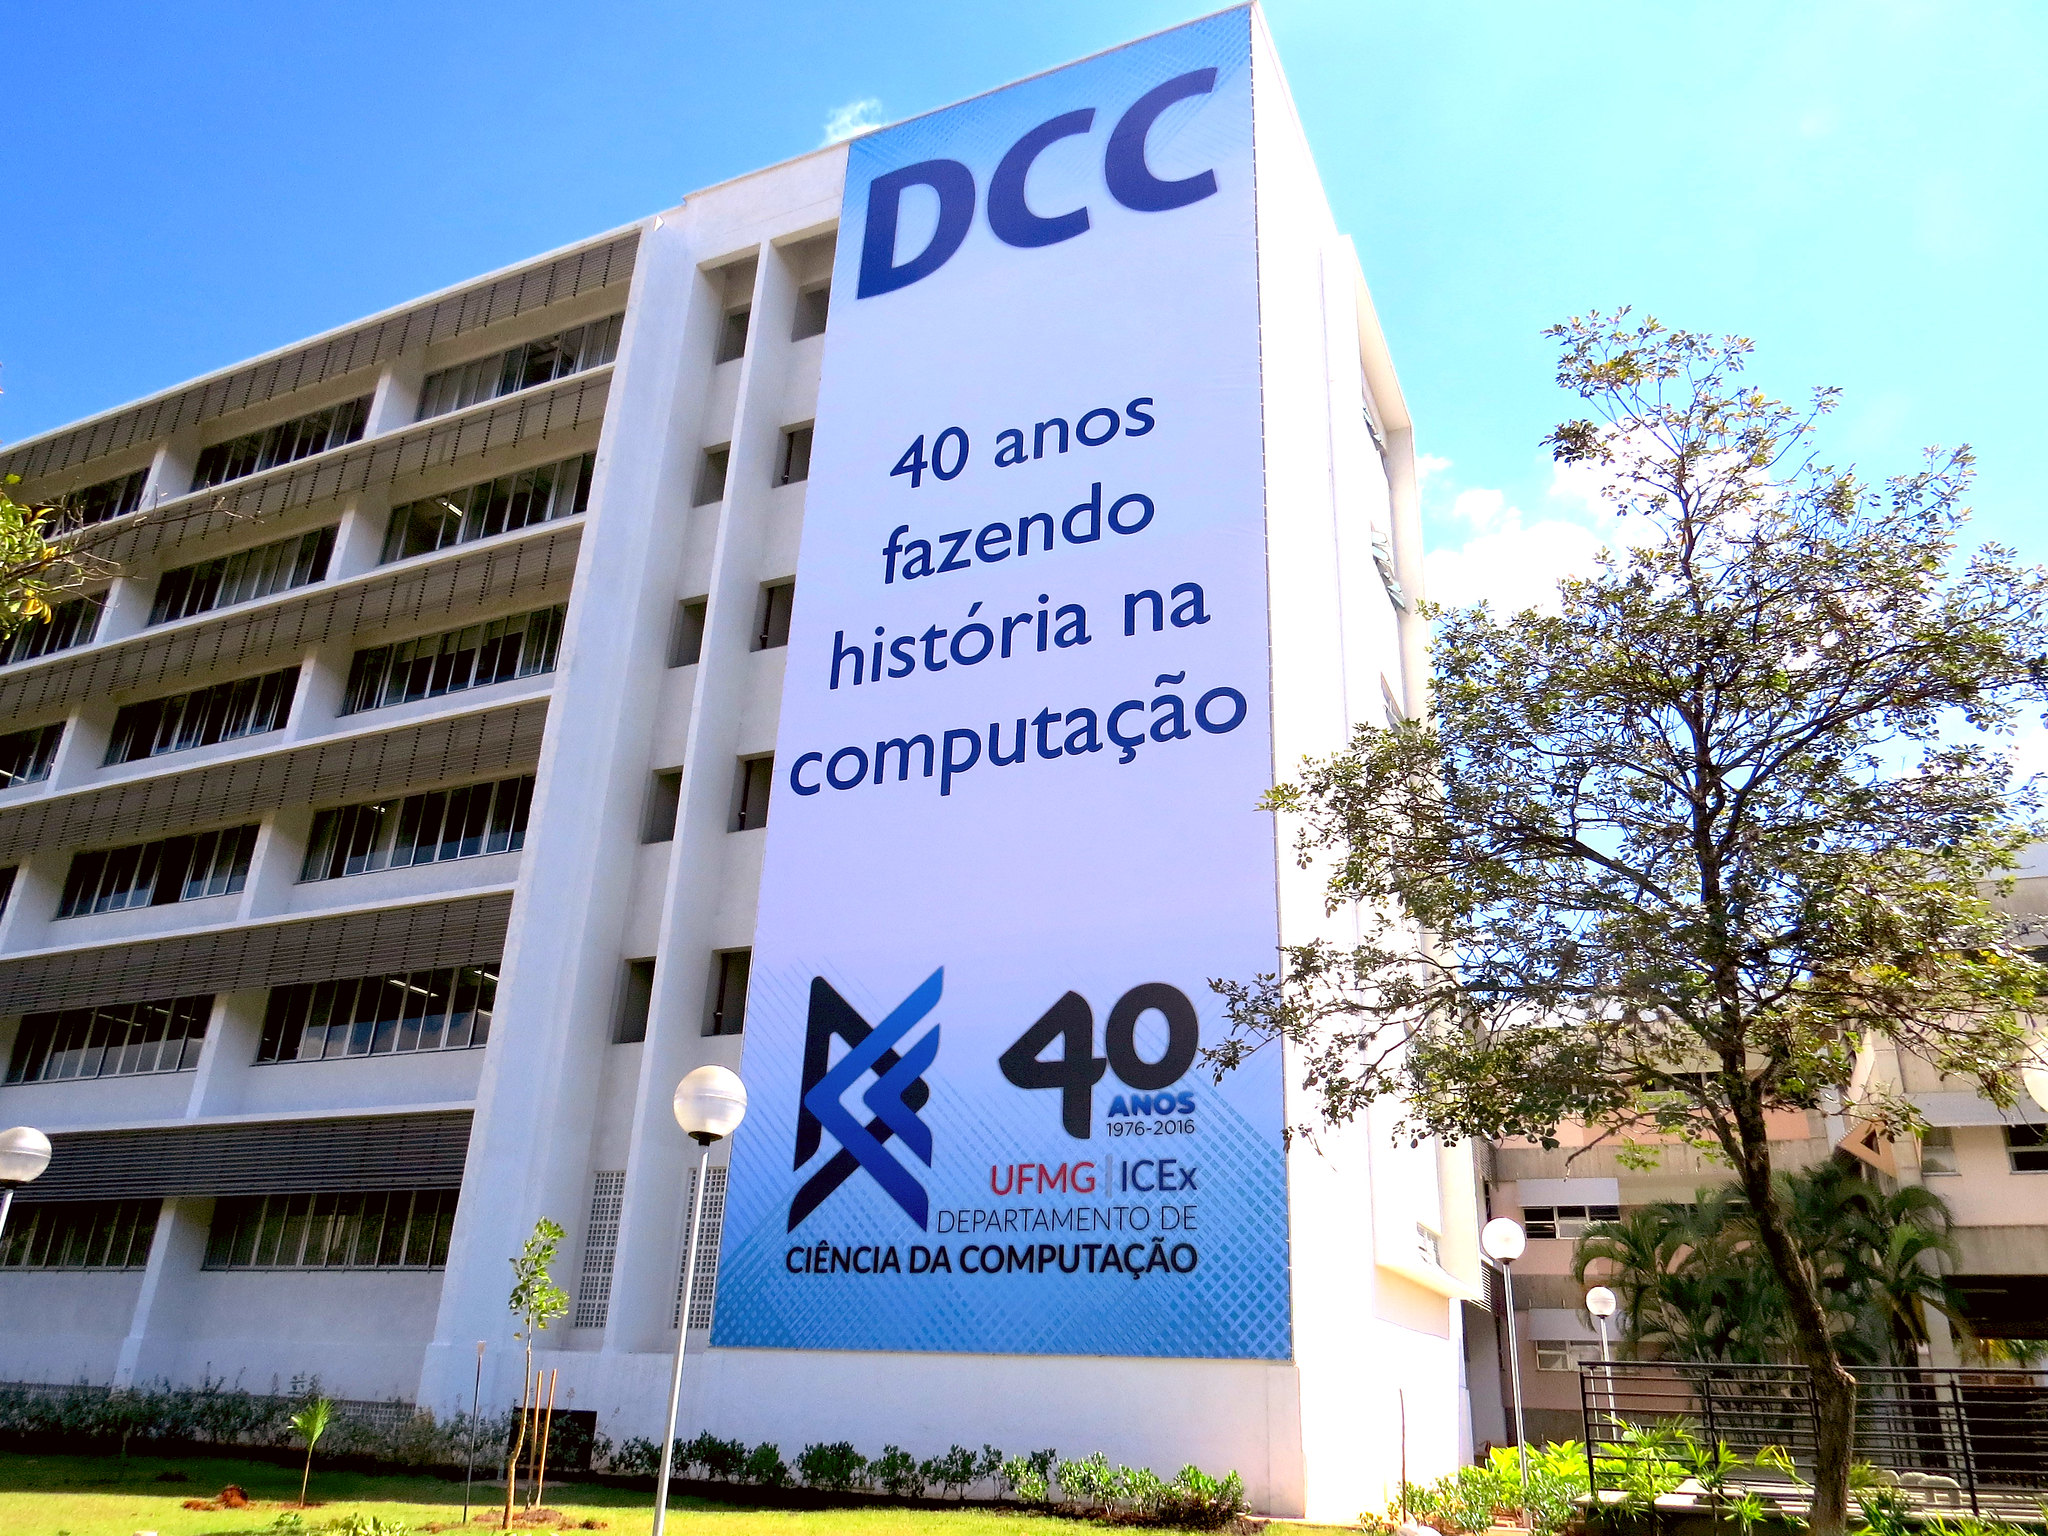
\includegraphics[width=\textwidth]{img/dcc.jpg}
	% 		\caption{Prédio do DCC em 2016.}
	% 		\label{fig:exemplo}
	% 	\end{figure}

	% 	\lipsum[5]

	% 	\begin{table}[h]
	% 		\centering
	% 		\begin{tabular}{c|ccccccccl}
	% 			Natural & \multicolumn{9}{c}{Real}   \\ \hline
	% 			1 & 0.  & {\color{red} 2}  & 3   & 6   & 4   & 3   & 6   & 7   & $\ldots$ \\
	% 			2  & 0.  & 0   & {\color{red} 9}  & 8   & 4   & 7   & 3   & 2   & $\ldots$ \\
	% 			3  & 0.  & 1   & 9   & {\color{red} 3}  & 2   & 1   & 4   & 0   & $\ldots$ \\
	% 			4  & 0.  & 8   & 4   & 3   & {\color{red} 2}  & 7   & 9   & 2   & $\ldots$ \\
	% 			5  & 0.  & 0   & 1   & 2   & 9   & {\color{red} 3}  & 4   & 8   & $\ldots$ \\
	% 			6  & 0.  & 2   & 8   & 2   & 6   & 5   & {\color{red} 8}  & 3   & $\ldots$ \\
	% 			7  & 0.  & 0   & 2   & 1   & 5   & 3   & 7   & {\color{red} 4}  & $\ldots$ \\
	% 			$\vdots$ & $\vdots$  & $\vdots$  & $\vdots$  & $\vdots$  & $\vdots$  & $\vdots$  & $\vdots$  & $\vdots$  & $\ddots$ \\ \hline
	% 			\multicolumn{1}{l|}{} & \multicolumn{1}{l}{0.} & \multicolumn{1}{l}{{\color{red} 2}} & \multicolumn{1}{l}{{\color{red} 9}} & \multicolumn{1}{l}{{\color{red} 3}} & \multicolumn{1}{l}{{\color{red} 2}} & \multicolumn{1}{l}{{\color{red} 3}} & \multicolumn{1}{l}{{\color{red} 8}} & \multicolumn{1}{l}{{\color{red} 4}} & $\ldots$
	% 		\end{tabular}
	% 		\caption{Cantor: Existem infinitos diferentes!}
	% 		\label{tab:exemplo}
	% 	\end{table}

	% 	\section{Usando referências}
	% 		Segundo \cite{horn86robot}, todo triângulo equilátero tem os lados iguais. Já segundo \cite{shashua97photometric}, todo quadrado também tem.

	% 		Veja que o pacote \verb|natbib| permite uma série de formas diferentes para fazer referências bibliográficas. O comando padrão, \verb|\cite|, realiza a citação comum vista no parágrafo anterior. Outros comandos permitem, por exemplo, colocar automaticamente a citação entre	parênteses \citep{hougen93estimation, sato99illumination2, sato99illumination1, sato01stability}.

	% 		O comando usado foi \verb|\citep|. Veja a documentação do \verb|natbib| na Internet para conhecer	outros comandos e exemplos de uso.

	% 		Citações aleatórias para fazer com que as referências bibliográficas ocupem	mais de uma página: \cite{bichsel92simple, dror01statistics, guisser92new, dwork2006calibrating, sweeney2002k}.

		%% Referências
		\bibliographystyle{plain}
		\bibliography{referencias}

		% \begin{apendices}
		% 	\chapter{Um apêndice}
		% 		\lipsum[1-3]

		% 	\chapter{Outro Apêndice}
		% 		\lipsum[4-6]

		% \end{apendices}
		
\end{document}
